%%%%%%%%%%%%%%%%%%%%%%%%%%%%%%%%%%%%%%%%%%%%%%%%%%%%%%%
% MatPlotLib and Random Cheat Sheet
%
% Edited by Michelle Cristina de Sousa Baltazar
%
% http://matplotlib.org/api/pyplot_summary.html
% http://matplotlib.org/users/pyplot_tutorial.html
%
%%%%%%%%%%%%%%%%%%%%%%%%%%%%%%%%%%%%%%%%%%%%%%%%%%%%%%%

\documentclass[a4paper]{article}
\usepackage[landscape]{geometry}
\usepackage{url}
\usepackage{multicol}
\usepackage{amsmath}
\usepackage{amsfonts}
\usepackage{tikz}
\usetikzlibrary{decorations.pathmorphing}
\usepackage{amsmath,amssymb}

\usepackage{colortbl}
\usepackage{mathtools}
\usepackage{amsthm, amsmath, amssymb, amsfonts}
\usepackage{enumitem}
\usepackage{fontawesome}
\usepackage[hidelinks]{hyperref}

%\title{Git Cheat Sheet}
\usepackage[english]{babel}
\usepackage[utf8]{inputenc}
\usepackage{bm}

\newcommand{\pd}[2]{\frac{\partial #1}{\partial #2}}
\newcommand{\loss}[0]{\mathcal{L}}
\newcommand{\chain}[3]{\frac{\partial #1}{\partial #2}\frac{\partial #2}{\partial #3}}
\newcommand{\eq}[1]{\begin{equation*}\begin{split}#1\end{split}\end{equation*}}
\newcommand{\coderef}[0]{Please find the implementation in the folder with the code files.}
\newcommand{\TODO}[1]{\textbf{\textcolor{red}{#1}}}

%%%%%%%%%%%%%%
% Shades of purple colors
%%%%%%%%%%%%%%
\usepackage{xcolor}

% Define colors
\definecolor{background}{HTML}{2D2B55}
\colorlet{boxcolor}{background!90}
\definecolor{textcolor}{HTML}{FFFFFF} %{FFFFFF}  %{B362FF}

\definecolor{goldenyellow}{HTML}{FAD000}  % FFEE80
\definecolor{lightyellow}{HTML}{FFEE80} 
\definecolor{lightpurple}{HTML}{A599E9}
\definecolor{brightpurple}{HTML}{4D21FC} %{B362FF} % 4D21FC
\definecolor{brightgreen}{HTML}{3AD900}
\definecolor{icyblue}{HTML}{9EFFFF}
\definecolor{deeppink}{HTML}{FF628C}
\definecolor{icypink}{HTML}{FB94FF}
\definecolor{paleyellow}{HTML}{FAEFA5}
\definecolor{orange}{HTML}{FF9D00}
\colorlet{linkcolor}{lightyellow}


\geometry{left=0.5cm,right=0.5cm,top=0.25cm,bottom=1.5cm}

% Apply to document
\pagecolor{background}
\color{textcolor}

\hypersetup{
	colorlinks=true,
	linkcolor=linkcolor,
	urlcolor=linkcolor,
}
%%%%%%%%%%%%%%

%%%%%%%%%%%%%%
%     Make a footer
%%%%%%%%%%%%%%
\usepackage{fancyhdr}
\usepackage[absolute,overlay]{textpos}
\pagestyle{fancy}

\fancyfoot{}  % Clear all footer fields
\fancyfoot[R]{ 
	\textcolor{lightpurple}{\small{
	\href{https://github.com/bellanich}{\faGithub{} {bellanich}} \hspace{0.3cm}
	\href{https://github.com/bellanich}{\faLinkedinSquare{} {bellanich}}
	}}
}
%%%%%%%%%%%%%%

\parindent0pt
\parskip2pt


\begin{document}


%%%%%%%%%%%%%%%
%      TITLE
%%%%%%%%%%%%%%%
\begin{center}
	\textcolor{lightpurple}{
		\textbf{\LARGE{Git Cheat Sheet}}\\
	}
\end{center}
%%%%%%%%%%%%%%%



%%%%%%%%%%%%%%%
%      Cheat Sheet Body
%%%%%%%%%%%%%%%
\footnotesize
\begin{multicols*}{3}

\tikzstyle{mybox} = [draw=black, fill=white, very thick,
    rectangle, rounded corners, inner sep=10pt, inner ysep=10pt]
\tikzstyle{fancytitle} =[fill=black, text=white, font=\bfseries]



\colorlet{outlinecolor}{icypink}

\begin{tikzpicture}
	\node [mybox, fill=boxcolor, draw=outlinecolor] (box){%
		\begin{minipage}{0.3\textwidth}
			\vspace{0.1cm}
			\underline{Source control} is the practice of tracking and managing changes to code. There are two types:
			\begin{enumerate}
				\item In \textcolor{outlinecolor}{centralized source control}, a centralized server acts as the ultimate source of truth for a collection of versioned files. 
				\begin{itemize}
					\item \textit{Implications.} An internet connection to the central server is required for most basic operations.
					\item \textit{Examples.} \href{https://subversion.apache.org}{Subversion}, \href{https://cvs.nongnu.org}{CVS}
				\end{itemize}
				\item \textcolor{outlinecolor}{Distributed or decentralized source control} doesn't require a central source of truth and allows for most operations to be local.
				\begin{itemize}
					\item \textit{Implications.} You can work independently of an internet connection.
					\item \textit{Examples.} Git, Mercurial (Hg)
				\end{itemize}
			\end{enumerate}
			\vspace{-3mm}
%			\begin{itemize}[leftmargin=4mm]
%				\setlength\itemsep{0.0em}
%				\item Neural Network is a directed acyclic graph
%				% \item Every module can be expressed by $a=h(x;w)$
%				\item Use loss function that matches output distribution to improve numerical stability and make gradients larger
%				\item Input and output distribution of every module should be the same to prevent inconsistent behavior and harder learning
%			\end{itemize}
%			\underline{Backprop}: chain rule $\pd{z}{x_i}=\sum_j \chain{z}{y_j}{x_i}$, $\nabla_{\bm{x}} \bm{z} = \left(\pd{\bm{y}}{\bm{x}}\right)^T \cdot \nabla_{\bm{y}} \bm{z}$
%			\vspace{-1mm}
%			\begin{enumerate}[leftmargin=4mm, label=\arabic*.]
%				\setlength\itemsep{0.2em}
%				\item Compute forward: $a^{(l)} = h^{(l)}\left(x^{(l)}\right)$, $x^{(l+1)}=a^{(l)}$
%				\item Compute reverse: $\pd{\loss}{a^{(l)}} = \left(\pd{a^{(l+1)}}{x^{(l+1)}}\right)^T \cdot \pd{\loss}{a^{(l+1)}}$\\
%				$\pd{\loss}{\theta^{(l)}} = \pd{a^{(l)}}{x^{(l+1)}} \cdot \left(\pd{\loss}{a^{(l)}}\right)^T$
%				\item Update params: $\theta^{(l)}_{t+1} = \theta^{(l)}_{t}-\eta \nabla_{\theta_t^{(l)}}\loss$
%			\end{enumerate}
		\end{minipage}
	};
	\node[fancytitle, right=10pt, fill=outlinecolor, text=black, draw=outlinecolor, rounded corners] at (box.north west) {History of Git};
\end{tikzpicture}


\colorlet{outlinecolor}{orange}

\colorlet{headercolor}{outlinecolor}
\colorlet{rowcolor1}{outlinecolor!90}
\colorlet{rowcolor2}{outlinecolor!70}

\begin{tikzpicture}
	\node [mybox, fill=boxcolor, draw=outlinecolor] (box){%
		\begin{minipage}{0.3\textwidth}
			\vspace{0.1cm}
			\textcolor{outlinecolor}{A repository} is a collection of version controlled files that are kept together. This includes \textbf{(a)} all the files related to a specific project/application, \textbf{(b)} the history of changes, and \textbf{(c)} any special configurations. \\
			
			\vspace{-1mm}
			\underline{Git states}: Git has three \textbf{local} states.
			\begin{enumerate}
				\item The \textcolor{outlinecolor}{working directory state} holds all the project or application files. These files may or may not be managed by Git, but Git is aware of them.
				\item The \textcolor{outlinecolor}{staging area state} or \textcolor{outlinecolor}{Git index state} is holding area for the queue of changes to be included in your next commit.
				\item The \textcolor{outlinecolor}{local Git repository state}  is a hidden folder called \inlinebash{.git}, which contains your entire local commit history.
			\end{enumerate}
			Git also has a \textcolor{outlinecolor}{remote (repository) state}, which is just another repository with its own three internal states. A specific Git command is used to move files between these states. i.e., \\
			
			\begin{minipage}{\textwidth}
				\centering
%				\vspace{-2mm}
				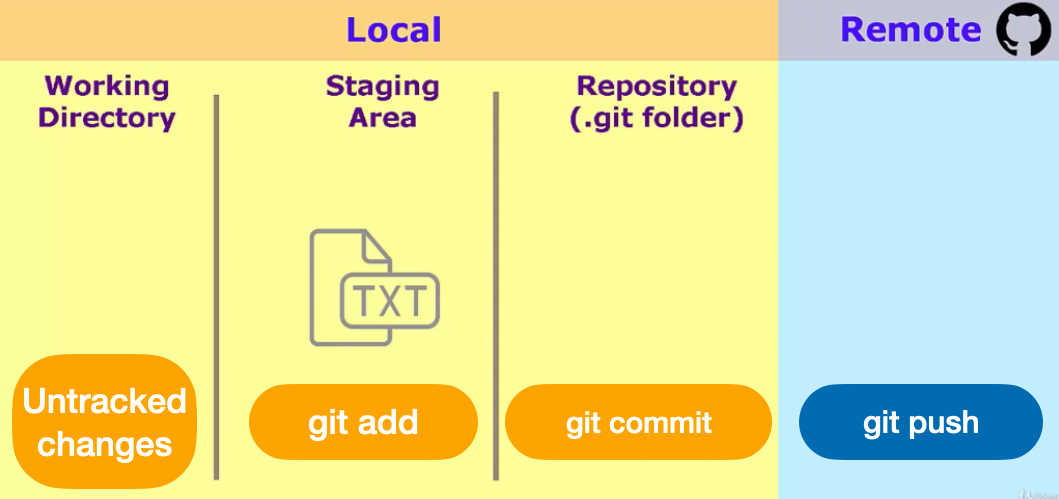
\includegraphics[width=0.5\textwidth]{images/git_stages.png}
				\vspace{-2mm}
				\captionof{figure}{Git states and associated commands. \href{https://www.udemy.com/course/git-complete/}{ \faLink{}  Source}}
			\end{minipage}
			
		\vspace{-3mm}
		\end{minipage}
	};
	\node[fancytitle, right=10pt, fill=outlinecolor, text=background, draw=outlinecolor, rounded corners] at (box.north west) {Git Basics};
\end{tikzpicture}
\begin{tikzpicture}
	\node [mybox, fill=boxcolor, draw=outlinecolor] (box){%
		\begin{minipage}{0.3\textwidth}
			\vspace{0.1cm}
			A \textcolor{outlinecolor}{tracked file}  is any file that Git is aware of and is actively tracking. i.e., Files that aren't new.
			

		\begin{center}
			\textcolor{background}{
				    \begin{tabularx}{\textwidth}{>{\columncolor{rowcolor1}}X|>{\columncolor{rowcolor2}}p{5cm}}
					\arrayrulecolor{boxcolor} % Set color of table rules
					\rowcolor{headercolor} % Color of the header row
					\textbf{Column A} & \textbf{Column B} \\ % Bold and center the header text
					\hline % Add a horizontal line below the header row
					A & A long text that will wrap to the next line \\
					\rowcolor{rowcolor2} % Color of the second row
					C & D \\
				\end{tabularx}
%		    	\begin{tabularx}{\textwidth}{>{\columncolor{rowcolor1}}X|>{\columncolor{rowcolor2}}p{5cm}}
%					\arrayrulecolor{boxcolor} % Set color of table rules
%					\rowcolor{rowcolor1} % Color of the first row
%					A & A long text that will wrap to the next line \\
%					\rowcolor{rowcolor2} % Color of the second row
%					C & D \\
%				\end{tabularx}
			}
		\end{center}
			
		\end{minipage}
	};
	\node[fancytitle, right=10pt, fill=outlinecolor, text=background, draw=outlinecolor, rounded corners] at (box.north west) {Git Basics (2)};
\end{tikzpicture}


\end{multicols*}
%%%%%%%%%%%%%%%


\end{document}